\section{Šablonový tisk}
-popis depozice pájecích past, parametry procesu a šablony, čištění
šablony

\subsection{Popis}
Metoda nanášení podobná sítotisku, rozdíl je v tom, že namísto síta je použita do rámu upnutá kovová šablona s vytvořeným motivem (leptáním nebo laserem).

Jedná se kontaktní způsob tisku - šablona přímo doléhá na tištěný substrát či plošky.

Odskok šablony je proveden po nanesení celého motivu.

Tento způsob tisku je vhodný pro nanášení souvislých ploch, nikoliv však dlouhých a složitých čar. Proto se používá k vytváření kontaktních plošek a k nanášení pájecích past.

Tloušťka nanesené vrstvy je dána tloušťkou šablony

Tento způsob tisku je vhodný pro nanášení souvislých ploch, nikoliv však dlouhýcha
složitých čar. Proto se používá k vytváření kontaktních plošek a k nanášení pájecích
past.

Šablonový tisk je svou základní podstatou obdobou sítotisku. Rozdíl je
v provedení šablony, jejíž motiv určený k tisku je vytvořen v pevném
(tuhém) materiálu, kterým často bývá ocelová nebo bronzová planžeta
(např. CuSn6).

Je zřejmé, že tištěné motivy musí být natolik uzavřené plochy aby
nebyla narušena tuhost šablony. Rychlost odtrhu musí být dostatečná
proto, aby se šablona dobře oddělila od nanesené pasty a aby zůstal

\begin{figure}[h]
   \begin{center}
     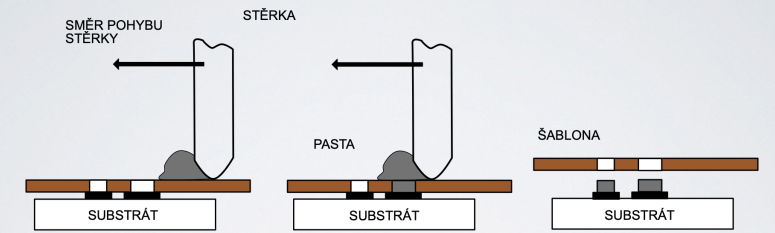
\includegraphics[scale=0.6]{images/SablonaTisk.png}
   \end{center}
   \caption{Šablonový tisk}
\end{figure}
\subsubsection{Výroba}
\textbf{Chemické leptání šablon:}Šablona se vytváří chemickým odleptáním plechu např. z nerezové oceli, kdy se na plech nanáší obraz z chemicky odolné látky, která
chrání místa, která nemají být odleptána. Šikmé hrany, které způsobují zatékání pasty (problém u jemných struktur).

\textbf{Laserové řezání šablon:} Šablony se vytváří řezáním pomocí laserového paprsku do kovové desky. Laser řeže otvory do kovové desky kontinuálně s lichoběžníkovými hrany
(s proměnnou kuželovitostí). Šablony jsou obecně drahé, velmi přesná metoda.

\textbf{Galvanoplastické šablony:}Šablony vytvořené touto metodou jsou nejlepší pro velmi jemné struktury a waferový tisk. Proces se skládá z nanášení niklu na fotoaktivní plastovou vrstvu pokovováním, která se mění působením světla na požadovaný obraz šablony.


\subsection{Parametry procesu a šablony}
\textbf{Šablona:} tloušťka šablony (definuje tloušťku nanesené pasty), materiál šablony\\
\textbf{Proces:} rychlost odtrhu, rychlost a tlak stěrky, její úhel

\subsection{Čištění}
Chemicky(rozpouštědla), mechanicky(ultrazvukem)